\documentclass[12pt]{beamer}
\usepackage{../latex-sty/mypres}
\usepackage[utf8]{inputenc}
\usepackage[T2A]{fontenc}
\usepackage[english]{babel}

\usefonttheme[onlymath]{serif}

\expandafter\def\expandafter\insertshorttitle\expandafter{%
  \insertshorttitle\hfill%
  \insertframenumber\,/\,\inserttotalframenumber}
\title[Seminar 11]{Optimization methods. \\
 Seminar 11. Intro to duality.}
\author{Alexandr Katrutsa}
\institute{Moscow Institute of Physics and Technology\\
Department of Control and Applied Mathematics} 
\date{\today}

\begin{document}
\begin{frame}
\maketitle
\end{frame}

\begin{frame}{Reminder}
\begin{itemize}
\item Existence solution of the optimization problem 
\item Optimality conditions for
\begin{itemize}
\item general optimization problem
\item unconstrained optimization problem
\item equality constrained optimization problem
\item equality and inequality constrained optimization problem 
\end{itemize}
\end{itemize}
\end{frame}

\begin{frame}{Notations}
\small
\begin{block}{Problem}
\vspace{-5mm}
\begin{equation*}
\begin{split}
& \min\limits f(x) = p^*\\
\text{s.t. } & g_i(x) = 0, \; i = 1,\ldots,m\\
& h_j(x) \leq 0, \; j = 1,\ldots, p
\end{split}
\end{equation*}
\end{block}

\begin{block}{Lagrangian}
\vspace{-2mm}
\begin{equation*}
L(x, \blambda, \bmu) = f(x) + \sum\limits_{i=1}^m\lambda_i g_i(x) + \sum\limits_{j=1}^p \mu_j h_j(x)
\vspace{-2mm}
\end{equation*}
\end{block}

\begin{block}{Dual variables}
Vectors $\bmu$ and $\blambda$ are called \emph{dual variables}.
\end{block}

\begin{block}{Dual function}
A function $g(\bmu, \blambda) = \inf\limits_x L(x, \blambda, \bmu)$ is called \emph{dual function}.
\end{block}

\end{frame}

\begin{frame}{Dual function properties}
\small
\begin{block}{Concavity}
The dual function is {\color{red}{concave}} as infimum of affine functions of $(\bmu, \blambda)$ independently of convexity of the primal problem.
\end{block}

\begin{block}{Lower bound}
For all $\blambda$ and for $\bmu \geq 0$ the following holds $g(\bmu, \blambda) \leq p^*$.
\end{block}

\begin{block}{Dual problem}
\vspace{-5mm}
\begin{equation*}
\begin{split}
& \max g(\bmu, \blambda) = d^*\\
\text{s.t. } & \bmu \geq 0
\end{split}
\end{equation*}
\end{block}

\begin{block}{What for?}
\begin{itemize}
\vspace{-2mm}
\item Dual problem is concave independently on convexity of primal problem
\vspace{-3mm}
\item Lower bound \textbf{can be} tight
\end{itemize}
\end{block}
\end{frame}

\begin{frame}{Conjugate function again}
Consider the problem
\begin{equation*}
\begin{split}
&\min f_0(x) \\
\text{s.t. } & \bA\bx \leq \mathbf{b}\\
& \bC\bx = \bd
\end{split}
\end{equation*}
Then
\begin{equation*}
\begin{split}
& g(\blambda, \bmu) = \inf_{\bx} (f_0(\bx) + \blambda^{\T}(\bA\bx - \mathbf{b}) + \bmu^{\T}(\bC\bx - \bd)) = \\
& - \mathbf{b}^{\T}\blambda - \bmu^{\T}\bd + \inf_{\bx}(f_0(\bx) + (\bA^{\T}\blambda + \bC^{\T}\bmu)^{\T}\bx) = \\
& - \mathbf{b}^{\T}\blambda - \bmu^{\T}\bd - f_0^*(-\bA^{\T}\blambda - \bC^{\T}\bmu)
\end{split}
\end{equation*}
Domains of dual and conjugate functions are related:
\[
\text{dom } g = \{ (\blambda, \bmu) \; | \; -\bA^{\T}\blambda - \bC^{\T}\bmu \in \text{dom } f^*_0 \}
\] 
\end{frame}

\begin{frame}{Examples}
Find dual function:
\begin{itemize}
\item Minimal norm solution of linear system 
\vspace{-3mm}
\begin{equation*}
\begin{split}
& \min \| \bx\|^2_2\\
\text{s.t. } & \bA\bx = \mathbf{b}
\end{split}
\end{equation*}
\item Linear programming
\vspace{-3mm}
\begin{equation*}
\begin{split}
& \min \bc^{\T}\bx\\
\text{s.t. } & \bA\bx = \mathbf{b}\\
& \bx \geq 0
\end{split}
\end{equation*}
\item Partitioning problem
\vspace{-3mm}
\begin{equation*}
\begin{split}
& \min \bx^{\T}\bW\bx\\
\text{s.t. } & x^2_i = 1, \; i = 1,\ldots,n
\end{split}
\end{equation*}
\end{itemize}
\end{frame}

\begin{frame}{Weak and strong duality}
\small
\begin{block}{Definition}
Optimal values of the primal objective and dual objective are related as 
%\vspace{-1mm}
\[
d^* \leq p^*.
\vspace{-2mm}
\]
If $d^* < p^*$, then \emph{weak} duality holds.

If $d^* = p^*$, then \emph{strong} duality holds.
\end{block}

\begin{block}{Remark}
Weak duality always holds by construction of the dual problem
\end{block}

\begin{block}{Questions}
\begin{itemize}
\item When the strong duality is hold?
\vspace{-3mm}
\item How to use duality to test optimality?
\end{itemize}
\end{block}
\end{frame}

\begin{frame}{Suboptimality criterion}
By construction $p^* \geq g(\blambda, \bmu)$, therefore $f_0(x) - p^* \leq f_0(x) - g(\blambda, \bmu) = \varepsilon$.
\begin{block}{Definition}
Difference $f_0(x) - g(\blambda, \bmu)$ is called \emph{duality gap} and gives upper bound for difference between current function value and optimal one.
\end{block}
How to use:
\begin{itemize}
\item stopping criterion in iterative process
\item theoretical estimate of convergence speed
\item check optimality of given point
\end{itemize}
\end{frame}

\begin{frame}{Slater's condition}
\begin{block}{Theorem}
If a problem is convex and there exists $x$ inside the interior of the feasible set, i.e. inequality constraints hold with strict inequalities, then the strong duality holds.
\end{block}

\begin{itemize}
\item Solution of linear system with minimum norm
\item Linear programming
\item Quadratically Constrained Quadratic Program (QCQP)
%\item Невыпуклая задача с сильной двойственностью
\end{itemize}
\end{frame}

\begin{frame}{Geometric interpretation}
\begin{center}
$\min\limits_{x} f_0(x), \text{ where } f_1(x) \leq 0.$
\end{center}
$
g(\lambda) = \inf\limits_{(u, t) \in \mathcal{G}} (t + \lambda u) \qquad \mathcal{G} = \{ (f_1(x), f_0(x)) \; | \; x \in \mathcal{D} \}
$

\begin{figure}
\centering
\includegraphics[scale=0.3]{dual_geometry.png}
\end{figure}
\begin{itemize}
\item $\lambda = 0$
\item $\lambda^*$~--- optimal value
\item $\lambda > \lambda^*$
\end{itemize}
\end{frame}

\begin{frame}{Complementary slackness condition}
Let $\bx^*$ and $(\bmu^*, \blambda^*)$ be solutions of the primal and dual problems, therefore
\begin{equation*}
\begin{split}
& f(\bx^*) = g(\bmu^*, \blambda^*) = \inf\limits_{\bx} L(\bx, \blambda, \bmu) \leq \\
& f(\bx^*) + \sum\limits_{i=1}^m\lambda^*_i g_i(\bx^*) + \sum\limits_{j=1}^p \mu^*_j h_j(\bx^*) \leq\\
& f(\bx^*), \qquad \bmu \geq 0 
\end{split}
\end{equation*}

\begin{block}{Complementary slackness condition}
\[
\mu^*_j h_j(\bx^*) = 0, \qquad j = 1,\ldots,p 
\]
For every inequality constraint:
\begin{itemize}
\item Lagrange multiplier is zero
\item inequality is active
\end{itemize} 
\end{block}
\end{frame}

\begin{frame}{KKT conditions}
From the last seminar we know KKT conditions: 
\begin{enumerate}
\item $g_i(x^*) = 0$~--- primal feasibility
\item $h_j(x^*) \leq 0$~--- primal feasibility
\item $ \mu^*_j \geq 0$~--- dual feasibility
\item $\mu^*_jh_j(x^*) = 0$~--- complementary slackness
\item $\nabla_x L(x^*, \blambda^*, \bmu^*) = 0$~--- stationariness of Lagrangian in primal variables
\end{enumerate}
Example $(\bP \in \mathbb{S}^n_+)$
\begin{equation*}
\begin{split}
& \min\limits_{\bx \in \bbR^n} \frac{1}{2}\bx^{\T}\bP\bx + \bq^{\T}\bx + r\\
\text{s.t. } & \bA\bx = \mathbf{b}
\end{split}
\end{equation*}
\end{frame}

\begin{frame}{Mechanical interpretation}
\begin{figure}
\centering
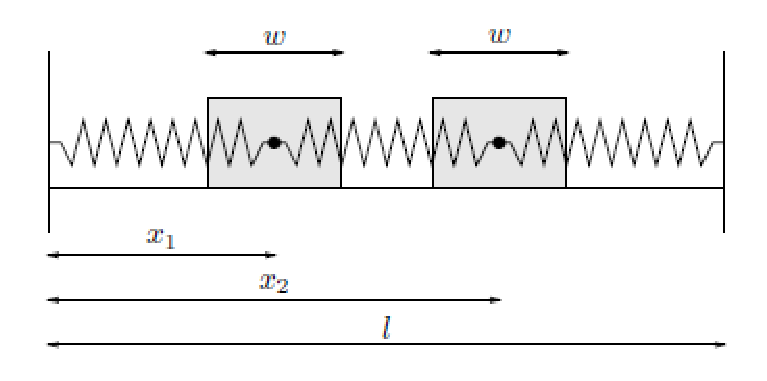
\includegraphics[scale=0.5]{kkt_mechanics.eps}
\end{figure}
Search equilibrium state of the system:
\begin{equation*}
\begin{split}
& \min_{\bx \in \bbR^3} \frac{1}{2}k_1x_1^2 + \frac{1}{2}k_2(x_2 - x_1)^2 + \frac{1}{2}k_3 (l - x_2)^2\\
\text{s.t. } & \frac{w}{2} - x_1 \leq 0\\
& w + x_1 - x_2 \leq 0\\
& \frac{w}{2} - l + x_2 \leq 0
\end{split}
\end{equation*}

\end{frame}

\begin{frame}{Examples}
\footnotesize
\begin{itemize}
\item Negative entropy with linear constraints
\vspace{-3mm}
\begin{equation*}
\begin{split}
& \min\limits_{\bx \in \bbR^n} \sum\limits_{i=1}^n x_i \log x_i\\
\text{s.t. } & \bA\bx \leq \mathbf{b}\\
& \mathbf{1}^{\T}\bx = 1
\end{split}
\end{equation*} 
\item State dual problem, solve it and recover solution of the primal problem from the dual solution:
\begin{equation*}
\begin{split}
& \min \frac{1}{2}x^2 + 2y^2 + \frac{1}{2}z^2 + x + y + 2z\\
\text{s.t. } & x+2y+z = 4
\end{split}
\end{equation*}
\item Lagrange relaxation for the binary linear programming problem:
\begin{equation*}
\begin{split}
&\min\limits_{\bx \in \bbR^n} \bc^{\T}\bx\\
\text{s.t. } & \bA \bx \leq \mathbf{b}\\
& x_i \in \{0,1 \}, \quad i = 1,\ldots,n
\end{split}
\end{equation*}
\end{itemize}
\end{frame}

\begin{frame}{Recap}
\begin{itemize}
\item Dual problem: what and why?
\item Weak and strong duality
\item Slater's condition
\item Geometrical and mechanical interpretations 
\end{itemize}
\end{frame}
\end{document}
